\section{Evaluation}
\label{sec: evaluation-hipster}

\begin{figure*}[htbp]
    \hspace{5mm}\begin{subfigure}[t]{0.45\textwidth}
    \centering        
    \begin{overpic}[width=\linewidth]{Chapter4/Figs/static-big-memcached-nolabel.eps}
        \put(40,95) {Memcached}
        \put(-5,15){\rotatebox{90}{Static mapping (all big cores)}}
        
     \end{overpic}
    \caption{Static mapping (all big cores)}
	\label{fig: Memcached-static}
\end{subfigure}%
    \hspace{2mm}\begin{subfigure}[t]{0.45\textwidth}
    \centering
    \begin{overpic}[width=\linewidth]{Chapter4/Figs/static-big-elasticsearch-nolabel.eps}
        \put(40,95) {Web-Search}
    \end{overpic}
    \caption{Static mapping (all big cores)}
	\label{fig:staticelasticsearch}
\end{subfigure}
    \hspace{5mm}\begin{subfigure}[t]{0.45\textwidth}
    \centering
        %\includegraphics
        \begin{overpic}[width=\linewidth]{Chapter4/Figs/octoman-memcached.eps}
            \put(-5,25){\rotatebox{90}{Octopus-Man}}
        \end{overpic}
  	\caption{Octopus-Man}
    \label{fig:octoman Memcached}
\end{subfigure}%
\hspace{2mm}\begin{subfigure}[t]{0.45\textwidth}
    \centering
    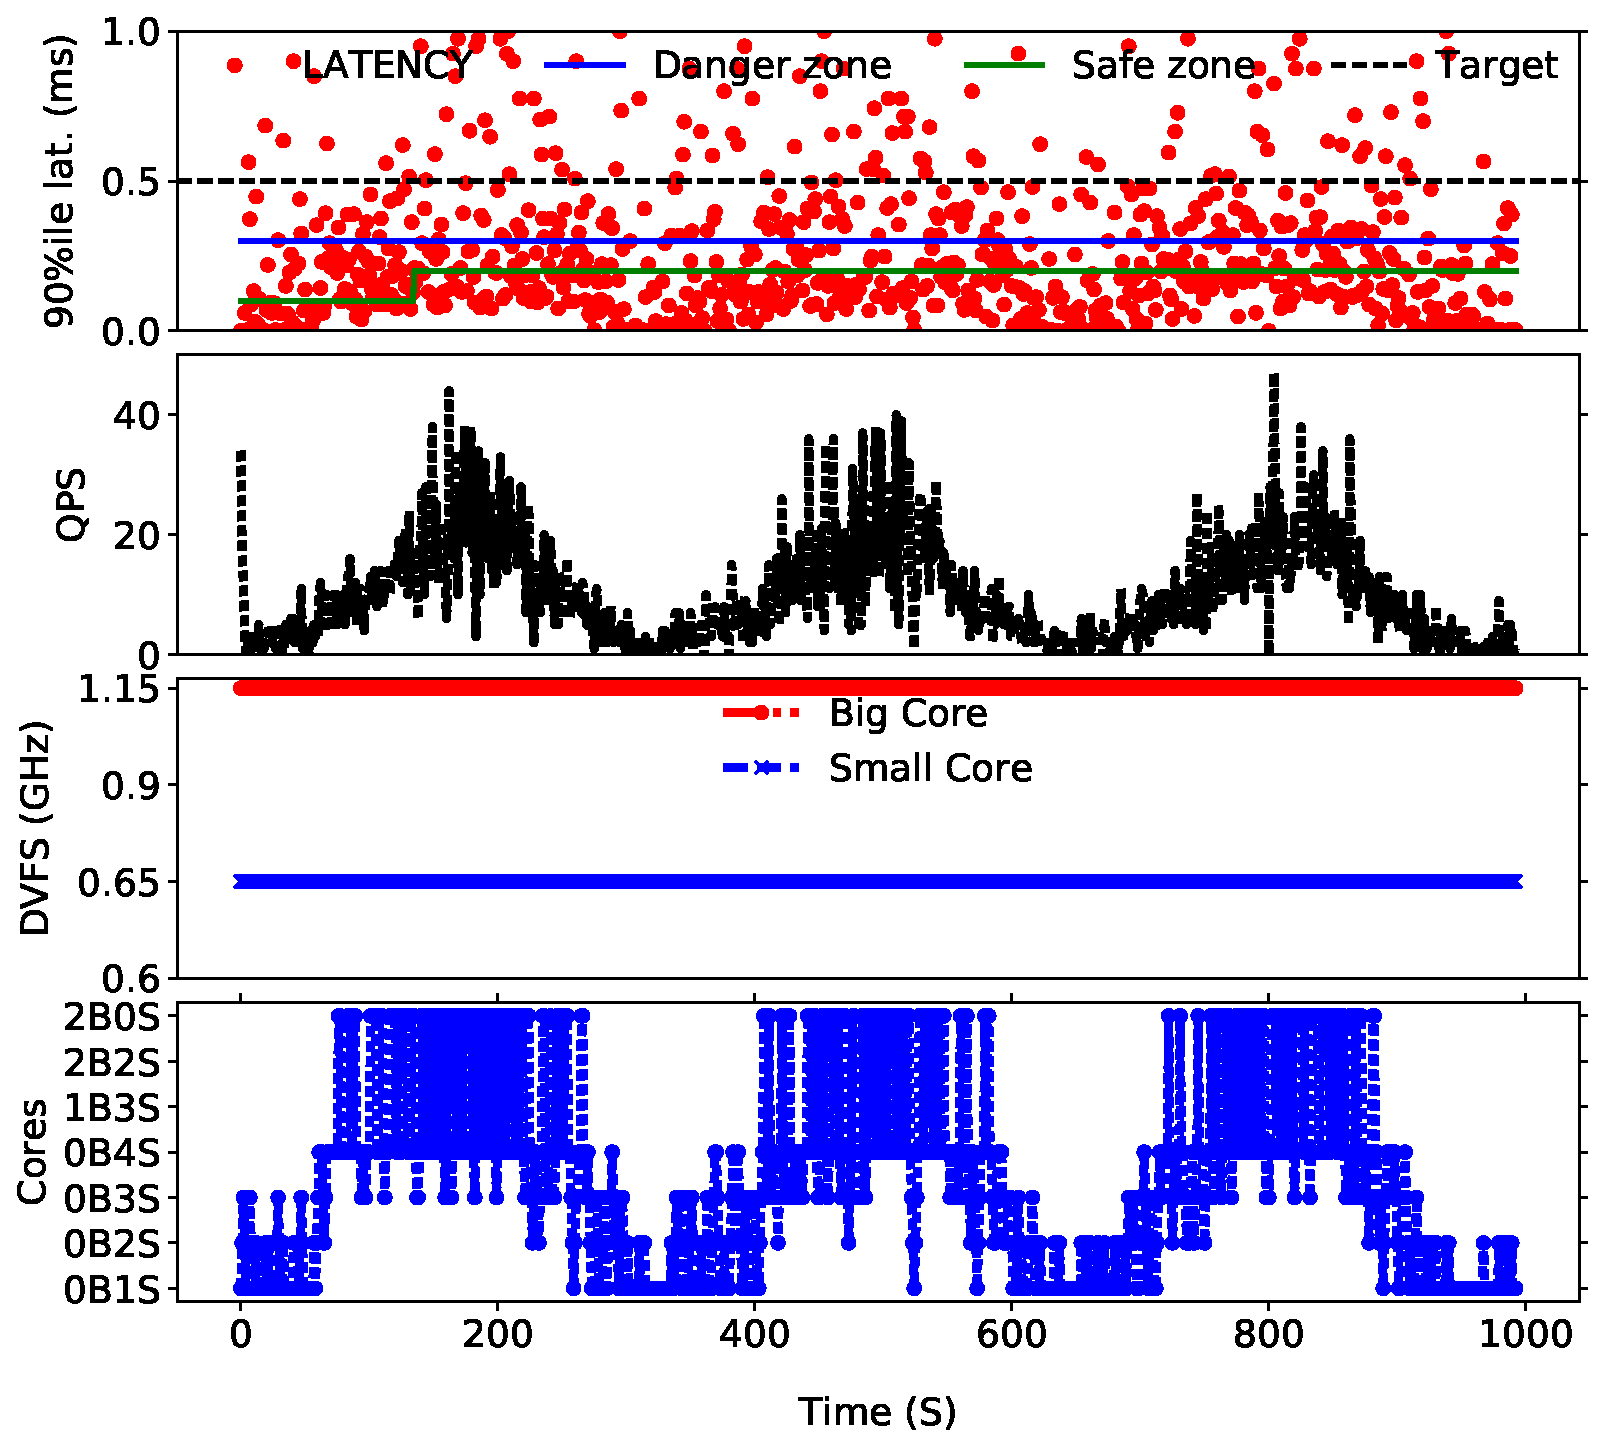
\includegraphics[width=\linewidth]{Chapter4/Figs/octoman-elasticsearch.eps}
  	\caption{Octopus-Man}
    \label{fig:octoman-elasticsearch}
\end{subfigure}
\hspace{5mm}\begin{subfigure}[t]{0.45\textwidth}
    \centering
        %\includegraphics
        \begin{overpic}[width=\linewidth]{Chapter4/Figs/memcached-heursitic.eps}
            \put(-5,15){\rotatebox{90}{Hipster's heuristic mapper}}
        \end{overpic}
    \caption{Hipster's heuristic mapper}
    \label{fig:Memcachedheuristic}
\end{subfigure}%
    \hspace{2mm}\begin{subfigure}[t]{0.45\textwidth}
	\centering
    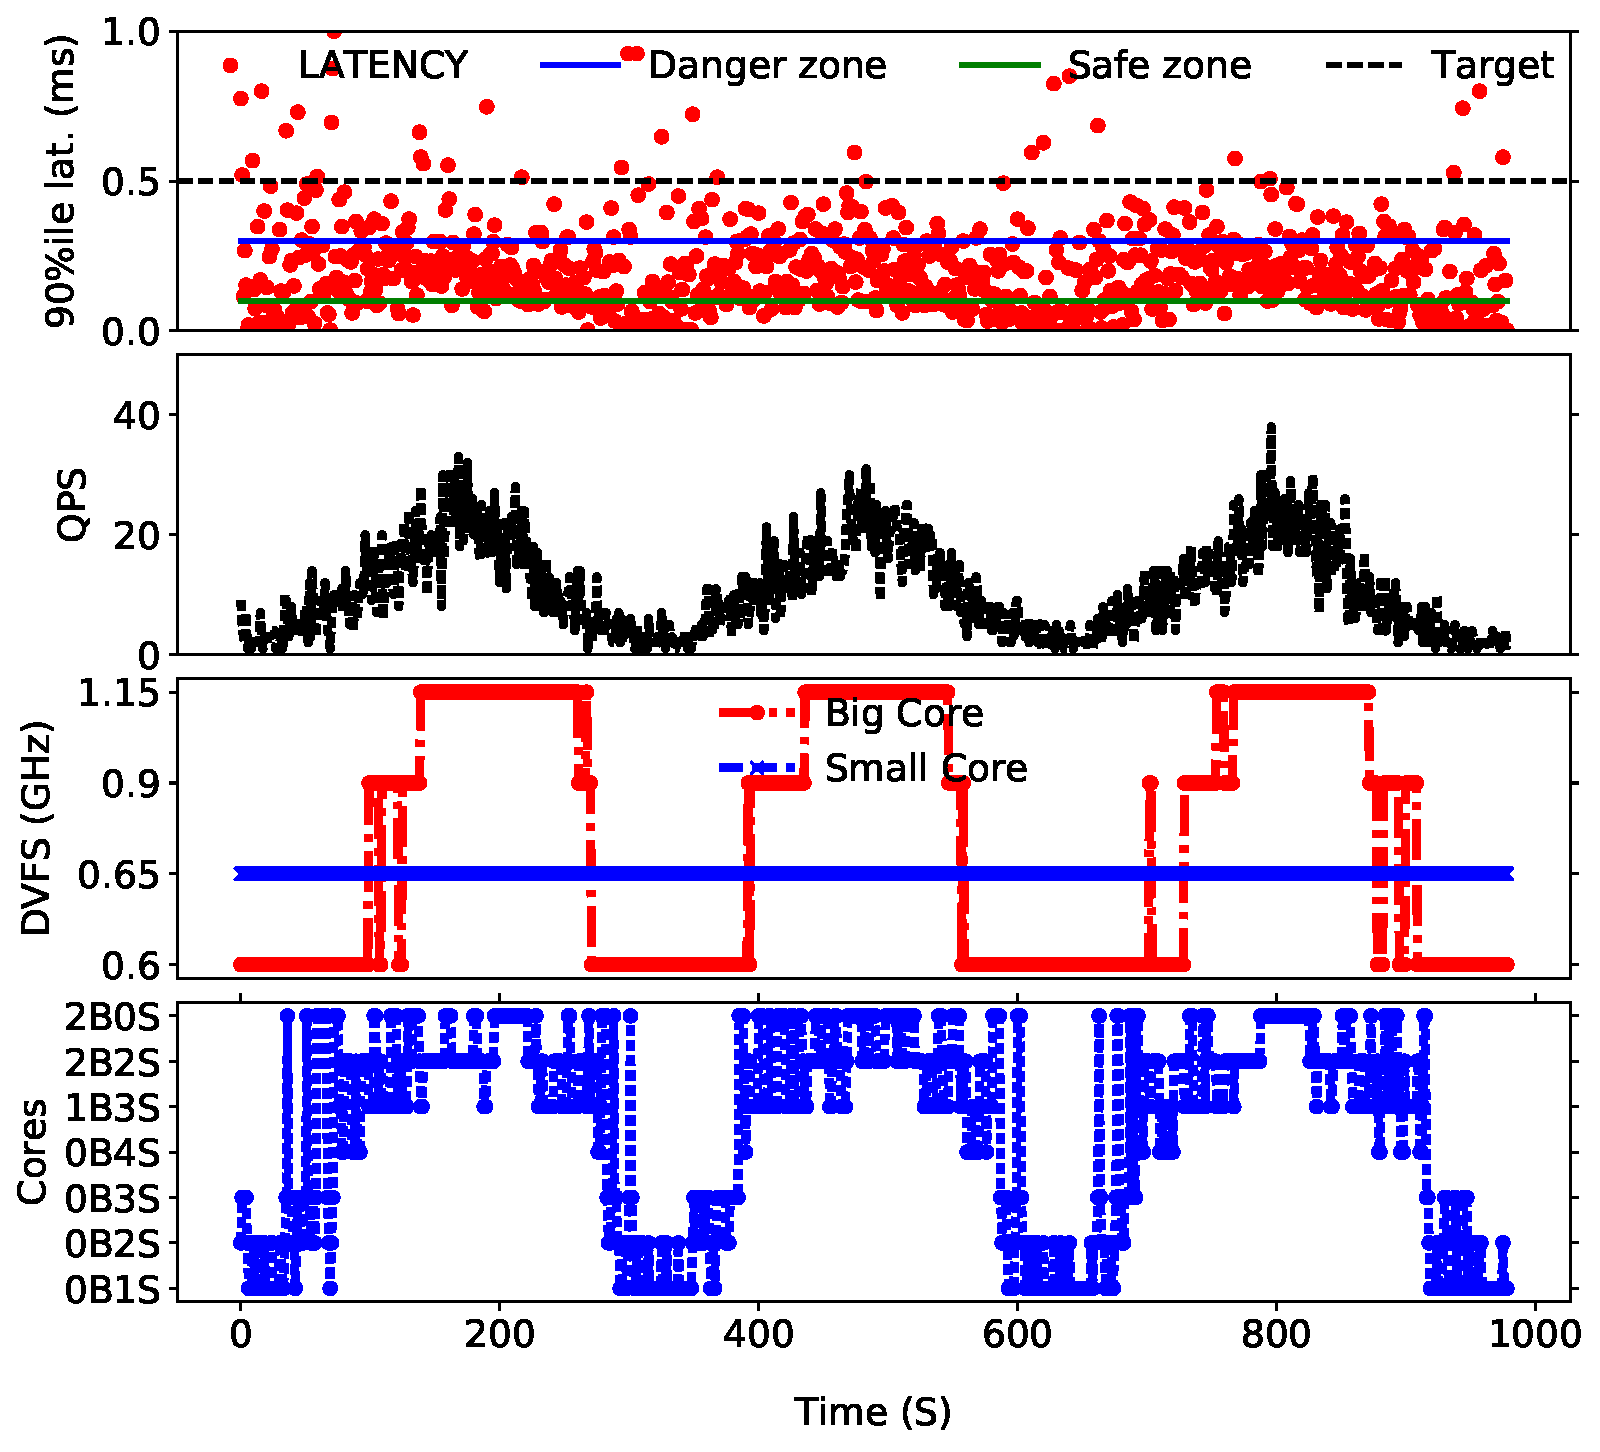
\includegraphics[width=\linewidth]{Chapter4/Figs/ourheuristic-es.eps}
	\caption{Hipster's heuristic mapper}
	\label{fig: ourheuristic-es}
\end{subfigure}
    \caption[Comparision of heuristic policies]{\captitle{Comparison of heuristic policies.} Static mapping (top), Octopus-Man (middle), and Hipster's heuristic policy (bottom). Results are shown for Memcached (left-hand column) and Web-Search (right-hand column) on ARM Juno R1.}
    %Hipster's heuristic policy (right-hand column) with static mapping (left) and Octopus-Man (centre). Results are shown for Memcached (top) and Web-Search (bottom) on ARM Juno R1.}
\label{fig:heuristic}
\end{figure*} 


\subsection{Algorithm Configuration}

In deploying Octopus-Man, we first performed a sweep on the danger and safe thresholds,
and picked the combination of thresholds with the highest QoS guarantee. For HipsterIn, we
set the learning phase to be 500~seconds, except when quantifying the learning time, where
we set it to 200~seconds. In addition, we quantify HipsterIn with changes in application
at runtime, where we run each application for 1500~seconds.



\subsection{HipsterIn Results} 
\label{subsec: results}

This section evaluates the effectiveness of HipsterIn, as a policy for managing a single
interactive workload.  The objective is to minimise system energy consumption while
satisfying QoS.

\subsubsection{Hipster's Heuristic Policy (interactive only)}
\label{subsubsec: heuristic interactive}

\looseness -1 We first evaluate the effectiveness of Hipster's heuristic policy alone, for
mapping interactive workloads. Figure~\ref{fig:heuristic} shows the results for both
workloads: Memcached (left-hand column , subfigures (a), (c) and (e)) and Web-search
(right-hand column, subfigures (b), (d) and (f)). The rows, from top to bottom, correspond
to static mapping, for which the interactive threads are mapped to the two big cores at
highest DVFS of \SI{1.15}{\giga\hertz} ((a) and (b)), Octopus-Man ((c) and (d)) and
Hipster's heuristic policy ((e) and (f)). For each subfigure, from top to bottom, the
first plot presents the tail latency (QoS), with the target marked with a dashed line.
The second plot shows the achieved throughput in RPS (requests per second). The third plot
presents the DVFS of the big and small cores, and the fourth plot represents the choice of
core mapping.

\looseness -1 Comparing the DVFS and core configuration subplots, we observe that
Hipster's heuristic policy is successfully exploring the DVFS settings available on the
Juno platform (bottom plots), and it is exploring all configurations including those that
use both big and small cores at the same time (bottom plots).  In contrast, Octopus-Man
does not adjust the DVFS settings and it uses either the big or small cores, but not both
at once. 

Both Octopus-Man and Hipster's heuristic policy frequently oscillate between consecutive
core configurations.  In the case of Octopus-Man, there are clear oscillations between two
big cores and four small cores, for example between the $600^{th}$ and $800^{th}$ seconds.
Using two big cores satisfies QoS but since it is within the safe zone, Octopus-Man
switches to four small cores, which enters the danger zone, generating an alert provoking
a return to two big cores. Such oscillations between cores in different clusters leads to
severe QoS degradation of up to \SI{20}{\percent}. As expected, the static mapping (all
big cores) has the least number of violations. 

\looseness -1 In summary, although Hipster's heuristic policy alone improves over
Octopus-Man by exploiting a wider search space, it still suffers from an unacceptable
number of QoS violations.

\begin{figure*}[b!]
\begin{minipage}[b]{.48\textwidth}
	\centering
	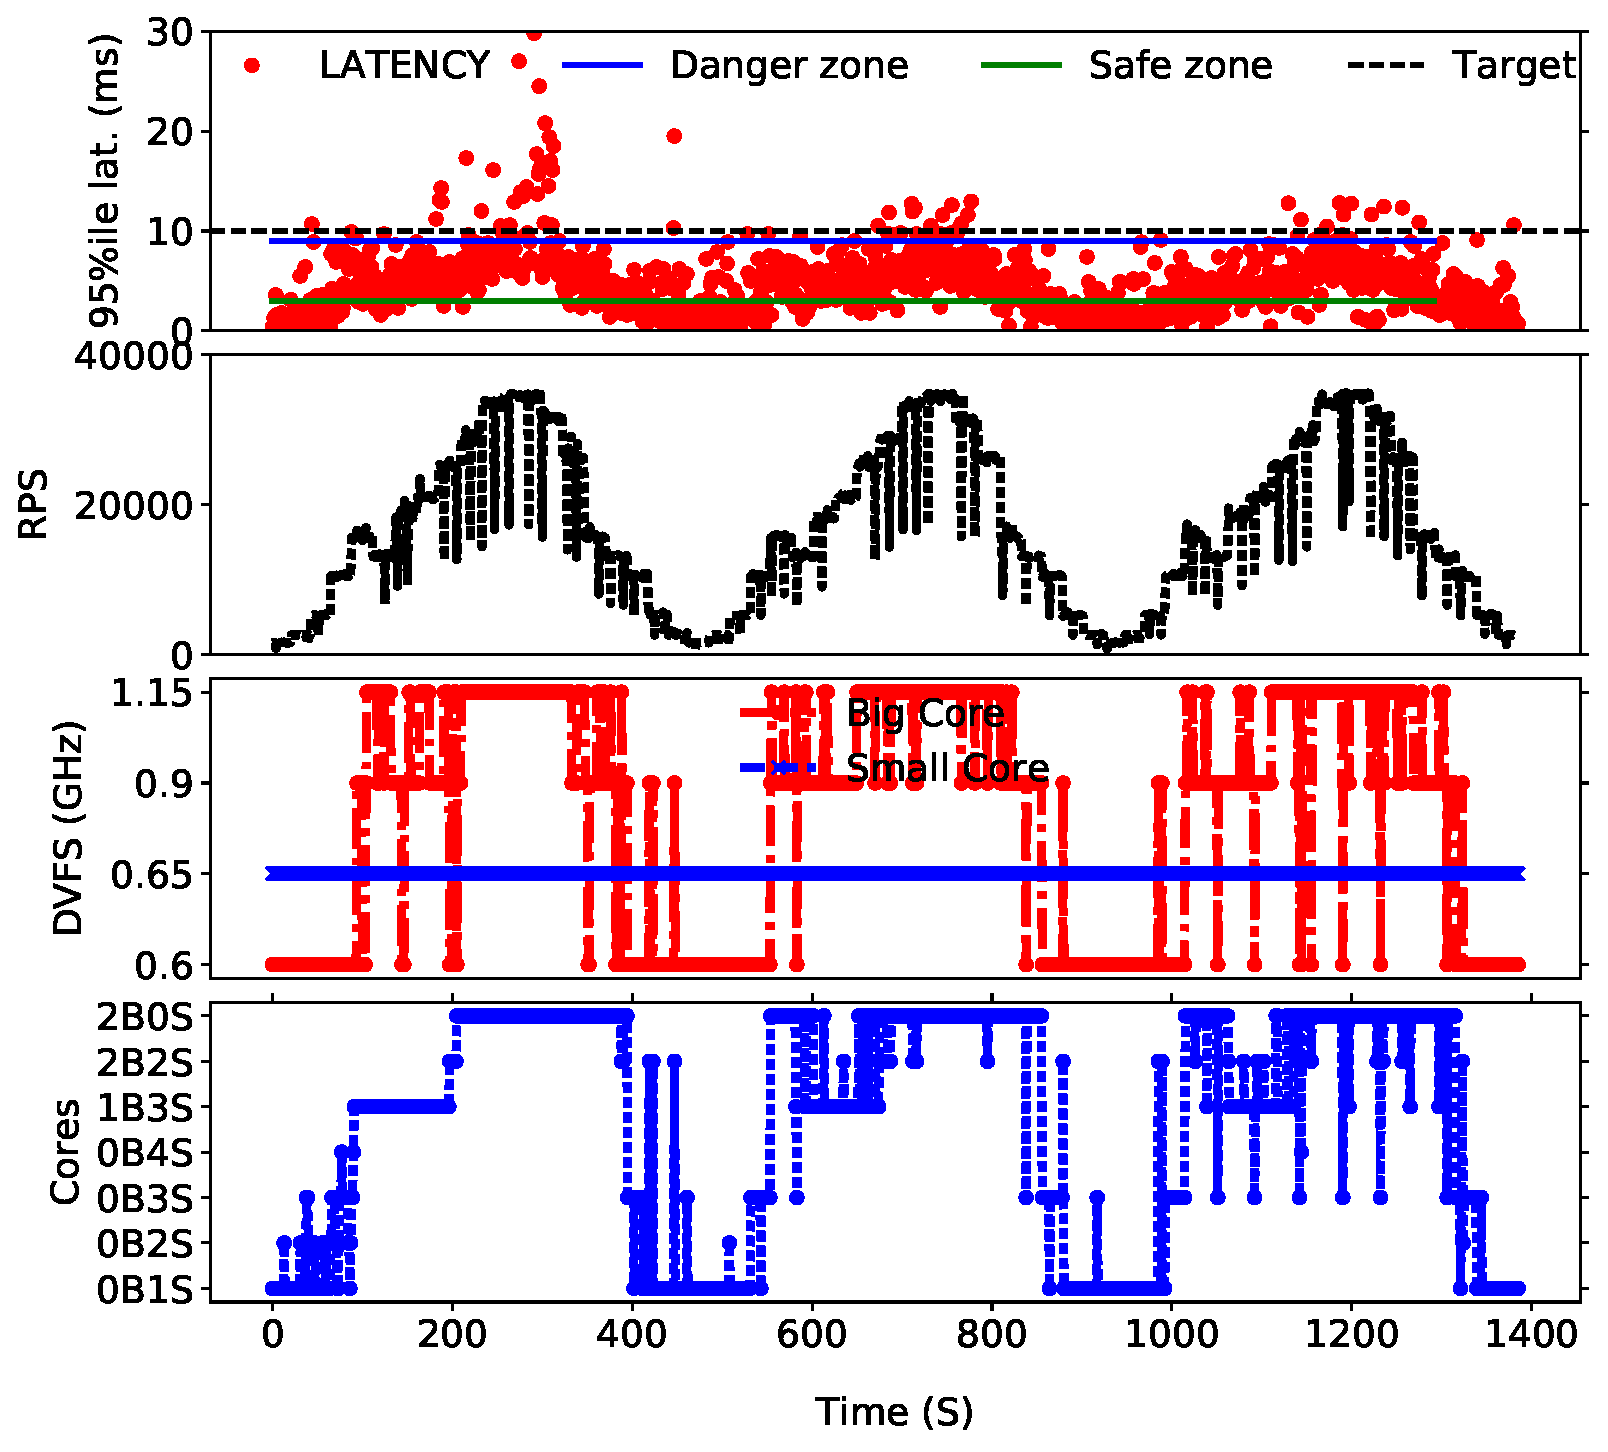
\includegraphics[width=\linewidth]{Chapter4/Figs/hipster-memcached-copy.eps}
    \caption[HipterIn on Memcached]{HipsterIn on Memcached}
    %\caption[HipterIn on Memcached]{HipsterIn on \\ \hspace*{19.5mm} Memcached}
	\label{fig: hipster-memcached} 
\end{minipage}
\hfill
\begin{minipage}[b]{.48\textwidth}
	\centering
	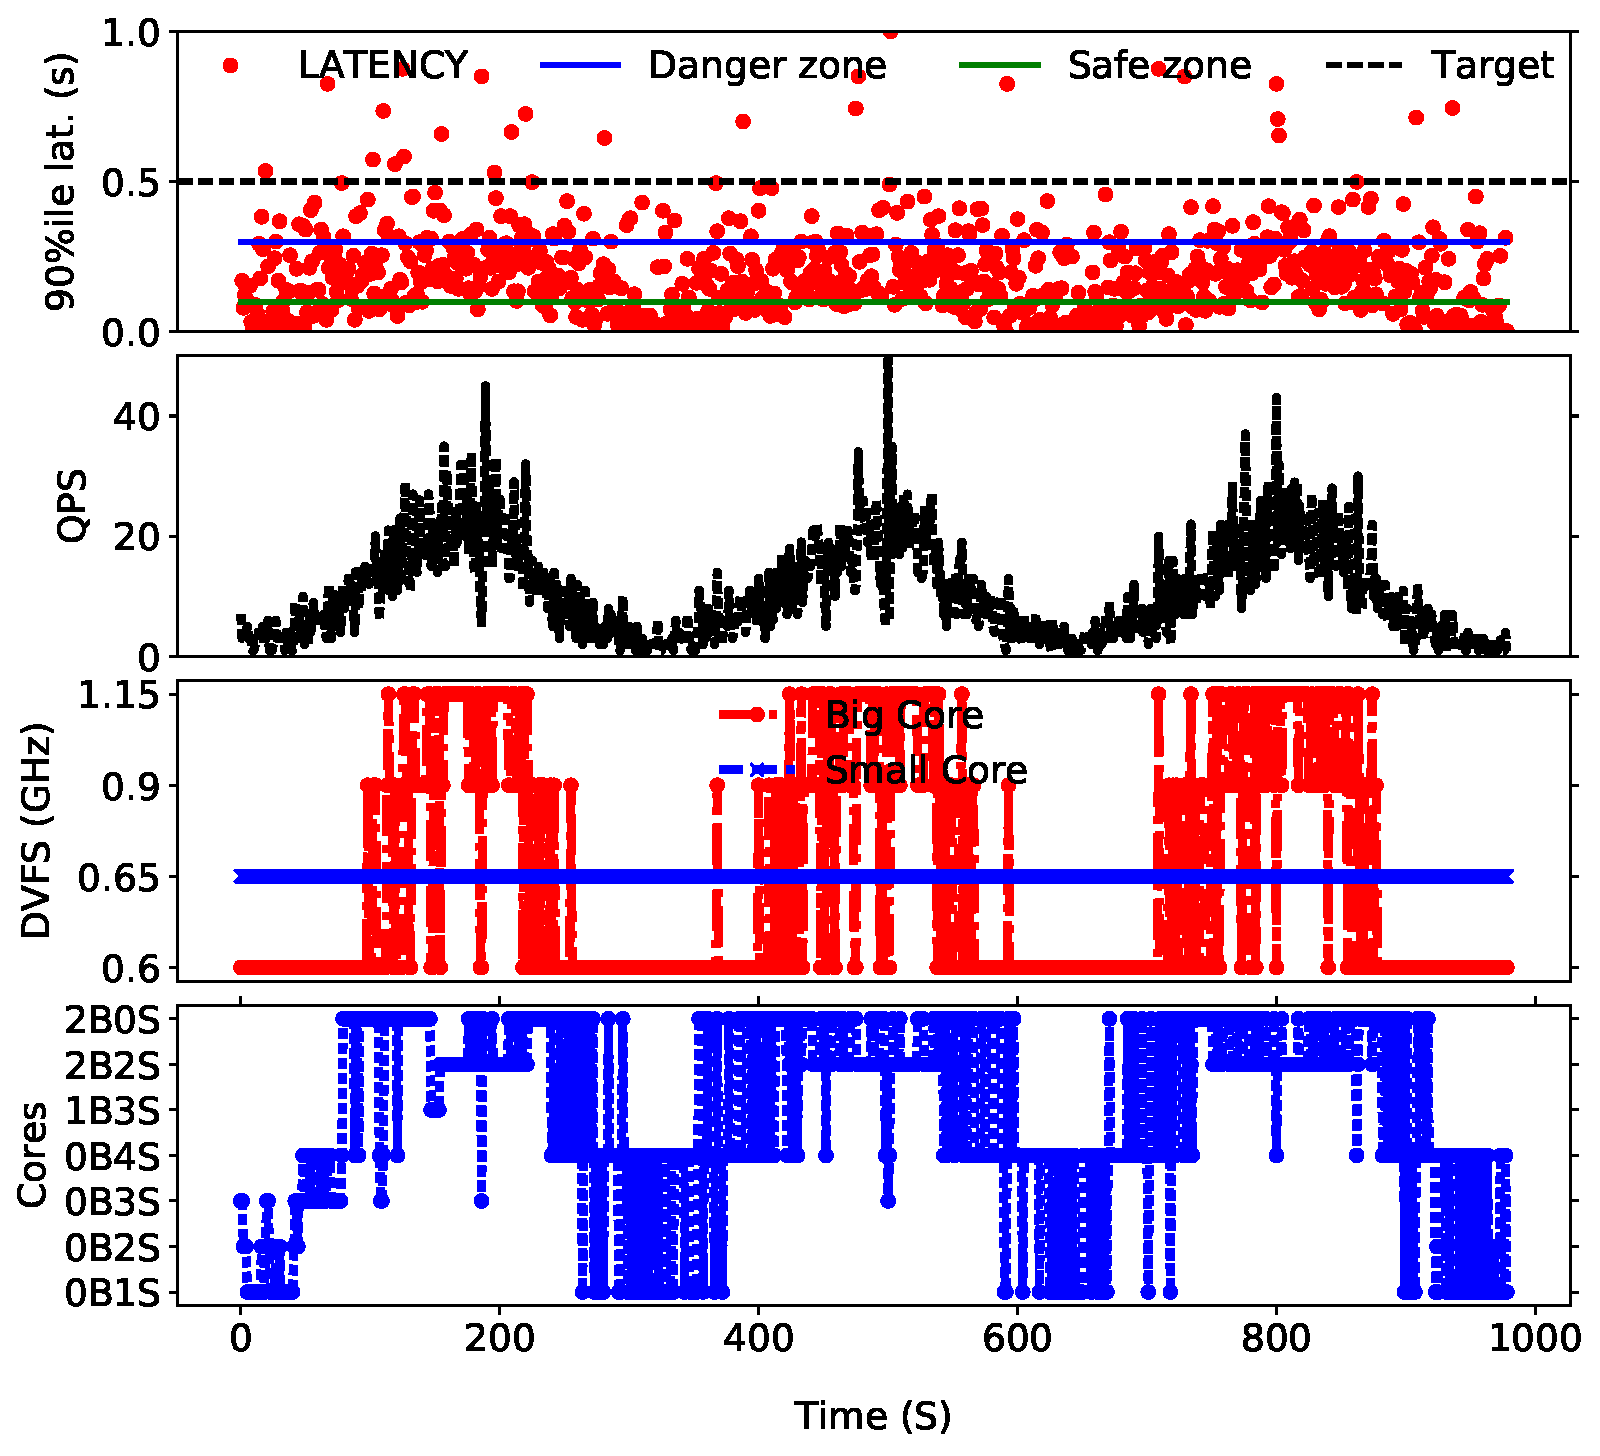
\includegraphics[width=\linewidth]{Chapter4/Figs/ril-elasticsearch.eps}
    \caption[HipsterIn on Web-Search]{HipsterIn on Web-Search}
    %\caption[HipsterIn on Web-Search]{HipsterIn on \\ \hspace*{19.5mm} Web-Search}
	\label{fig: hipster-elasticsearch}
\end{minipage}
\end{figure*}


\subsubsection{HipsterIn: Memcached Results}
\label{subsubsec: memcached results}

Figure~\ref{fig: hipster-memcached} shows the results using HipsterIn for Memcached.
After completing the learning phase, the oscillatory effect between core mappings is
greatly reduced (by \SI{8.3}{\percent}), and overall the QoS guarantee is improved by
\SI{24}{\percent} compared with the learning phase. HipsterIn performs well because it
moves directly to the appropriate core configuration for a given load that satisfies QoS. 

In addition to switching between a combination of different cores, HipsterIn also explores
more fine-grained DVFS adaptations, which has lower overheads (of microseconds) compared
with migrations between cores (order of milliseconds)~\citep{Kasture2015Rubik}.

\subsubsection{HipsterIn: Web-Search Results}
\label{subsubsec: web-search results}

Figure~\ref{fig: hipster-elasticsearch} shows the results using HipsterIn for Web-Search.
In contrast to the heuristic policies (Octopus-Man and Hipster's heuristic), during the
exploitation phase, HipsterIn monitors the QoS and dynamically adjusts the core mapping
and DVFS settings to adapt to load fluctuations. Both Hipster's heuristic and Octopus-Man
perform aggressive changes to core mappings to reduce energy, leading to a negative impact
on QoS. On the other hand, HipsterIn shows a more balanced behaviour, performing
$4.7\times$ fewer task migrations than Octopus-Man for Web-Search, while improving QoS up
to \SI{16}{\percent} and reducing energy consumption by \SI{13.5}{\percent}. 

\subsubsection{\textbf{HipsterIn: Swapping applications}}
\label{subsubsec: swap apps}

%We also evaluate the effectiveness of HipsterIn to adapt to changes in application with
%different characteristics at runtime.

We also evaluate the effectiveness of HipsterIn to adapt to changes in application at
runtime and deliver real-time performance guarantees even for the new incoming
application.

\paragraph*{Web-Search to Memcached} Figure~\ref{fig: hipster-elasticsearch-memcached}
shows the results using HipsterIn when swapping from Web-Search (represented in red) to
Memcached (represented in cyan) after \SI{1500}{\second} of execution. ``NA''
in the last two subplots on $y$-axis represents the period when Web-Search or Memcached are running
exclusively. HipsterIn shows a more balanced behaviour, performing 22\% fewer violations
than learning phase, set at 500-seconds, when running Web-Search. Thereafter, when
swapping Web-Search with Memcached observe that HipsterIn has a far more QoS violations
but quickly adapts to changes in application by learning the lookup table suitable for
Memcached.

\begin{figure*}[htb]
	\centering
    \begin{overpic}[width=\textwidth]{Chapter4/Figs/memcached-websearch.eps}
        \put(2.8,24.5){\tiny NA}
        \put(2.8,9.5){\tiny NA}
    \end{overpic}
	\caption{HipsterIn on Memcached swapping to Web-Search}
	\label{fig: hipster-memcached-websearch} 
\end{figure*}

\paragraph*{Memcached to Web-Search} Figure~\ref{fig: hipster-memcached-websearch} shows
the results using HipsterIn when swapping from Memcached (represented in cyan) to
Web-Search (represented in red) after \SI{1500}{\second} of execution. ``NA''
in the last two subplots on the $y$-axis represents the period when Memcached or Web-Search are running
exclusively.  When application is swapped at runtime from Memcached to Web-Search,
HipsterIn dynamically updates the lookup table to adapt to changes in application
behaviour. For instance, observe at \SI{1500}{\second}, HipsterIn has large number of
violations (by \SI{7.1}{\percent}) but quickly drops after it adapts the lookup table and
the overall QoS guarantee is improved by \SI{38}{\percent}. The QoS guarantee of HipsterIn for Web-Search is 95\%, which is similar to QoS guarantee when running Web-Search from the start (Table~\ref{tab: summarytable-hipster})

\begin{figure*}[htb]
	\centering
    \begin{overpic}[width=\textwidth]{Chapter4/Figs/websearch-memcached.eps}
        \put(2,24.5){\tiny NA}
        \put(2,9.5){\tiny NA}
    \end{overpic}
	\caption{HipsterIn on Web-Search swapping to Memcached}
	\label{fig: hipster-elasticsearch-memcached}
\end{figure*}




\subsubsection{HipsterIn Summary}
\label{subsubsec: summaryresults}

\iffalse
\begin{table*}[t]
\centering
%\ra{1.4}
\setlength{\tabcolsep}{2pt}
    \caption[Summary of HipsterIn for Memcached, and Web-Search]{\captitle{Summary of HipsterIn for Memcached and Web-Search.} A summary of QoS guarantees, tardiness and energy savings}
%\caption{HipsterIn: summary of QoS guarantees, tardiness and energy savings for Memcached and Web-Search.}
\scalebox{1}{
\begin{tabular}{@{}lrrcrrcrr@{}}\toprule
& \multicolumn{2}{c}{$QoS\enspace Guarantee$} & \phantom{abc}& \multicolumn{2}{c}{$QoS\enspace Tardiness$} & \phantom{abc} & \multicolumn{2}{c}{$Energy\enspace Reduction$}\\
\cmidrule{2-3} \cmidrule{5-6} \cmidrule{8-9}
& $Memcached$ & $Web-Search$ && $Memcached$ & $Web-Search$ && $Memcached$ & $Web-Search$ \\ 
\midrule
$Static\enspace$ (all big cores)   & 99.5\% & 99.5\%  && 1.1  & 1.3   && -       & -\\
$Static\enspace$ (all small cores) & 85.8\% & 78.4\%  && 1.4  & 2.0   && 48.0\% & 31.0\%\\
$Hipster's\enspace Heuristic$        & 89.9\% & 95.3\%   && 1.8  & 1.9   && 18.7\%  & 13.6\%\\
$OctopusMan$                   & 92.0\% & 80.0\%  && 2.2  & 2.1   && 17.2\%  & 4.3\%\\
$\textbf{HipsterIn}$             & \textbf{99.4\%} & \textbf{96.5\%} && 1.4  & 2.0 && \textbf{14.3\%}  & \textbf{17.8\%}\\
\bottomrule
\end{tabular}
}
\label{tab: summarytable-hipster}
\end{table*}
\fi

\begin{table*}[t]
\centering
%\ra{1.4}
\setlength{\tabcolsep}{2pt}
\caption[Summary of HipsterIn for Memcached, and Web-Search]{\captitle{Summary of HipsterIn for Memcached (Mem) and Web-Search (Web).} A summary of QoS guarantees, tardiness and energy savings}
%\caption{HipsterIn: summary of QoS guarantees, tardiness and energy savings for Memcached and Web-Search.}
\scalebox{0.95}{
\begin{tabular}{@{}lrrcrrcrr@{}}\toprule
& \multicolumn{2}{c}{$QoS\enspace Guarantee$} & \phantom{abc}& \multicolumn{2}{c}{$QoS\enspace Tardiness$} & \phantom{abc} & \multicolumn{2}{c}{$Energy\enspace Reduction$}\\
\cmidrule{2-3} \cmidrule{5-6} \cmidrule{8-9}
& $Mem$ & $Web$ && $Mem$ & $Web$ && $Mem$ & $Web$ \\ 
\midrule
$Static\enspace$ (all big cores)   & 99.5\% & 99.5\%  && 1.1  & 1.3   && -       & -\\
$Static\enspace$ (all small cores) & 85.8\% & 78.4\%  && 1.4  & 2.0   && 48.0\% & 31.0\%\\
$Hipster's\enspace Heuristic$        & 89.9\% & 95.3\%   && 1.8  & 1.9   && 18.7\%  & 13.6\%\\
$OctopusMan$                   & 92.0\% & 80.0\%  && 2.2  & 2.1   && 17.2\%  & 4.3\%\\
$\textbf{HipsterIn}$             & \textbf{99.4\%} & \textbf{96.5\%} && 1.4  & 2.0 && \textbf{14.3\%}  & \textbf{17.8\%}\\
\bottomrule
\end{tabular}
}
\label{tab: summarytable-hipster}
\end{table*}


Table~\ref{tab: summarytable-hipster} summarises the QoS guarantee, QoS tardiness and
energy reduction for Memcached and Web-Search for different policies: Static (all big
cores), Static (all small cores), Hipster's heuristic mapper, Octopus-Man and HipsterIn.
We compare the energy consumption of each mapping schema against Static (all big cores).
We quantify the QoS behaviour at each sampling interval by assessing the measured QoS
using two metrics: QoS guarantee and QoS tardiness.\footnote{QoS Tardiness is
$QoS_{\mathit{curr}}$/$QoS_{\mathit{target}}$, using the definitions from
Section~\ref{subsec: rewardcalculation}.} The QoS Guarantee is the percentage of  samples
for which the measured QoS did not violate the target (\SI{100}{\percent}-QoS
violations\%). The QoS tardiness in the table is the average (mean) of the QoS tardiness,
including only the samples that violated the QoS target.

As shown in Table~\ref{tab: summarytable-hipster}, for Web-Search and Memcached, static
(all small cores) cannot meet the required QoS. On the one hand, the heuristic policies
reduce energy marginally, but violate QoS due to excessive core migrations. On the other
hand, HipsterIn meets QoS at \SI{99.4}{\percent} and \SI{96.4}{\percent} for Memcached and
Web-Search, while having energy savings of \SI{14.3}{\percent} and \SI{17.8}{\percent},
respectively.



\subsubsection{HipsterIn Analysis}




\paragraph*{Rapid adaptation to load changes.} Hipster can respond to rapid changes in
load by directly mapping to a configuration that satisfies the QoS.  Figure~\ref{fig:
responsivenesstoloadchange} shows how HipsterIn (during the exploitation phase) and
Octo\-pus-Man respond to changes in load. From top to bottom, we express the input load in
terms of the percentage of maximum load, where it increases from \SI{50}{\percent} to
\SI{100}{\percent} over a period of 175 seconds for Memcached. In the second graph, we
express the \ninefive percentile tail latency as QoS Tardiness. A QoS violation has
occurred if the QoS Tardiness is above 1, otherwise QoS is satisfied.  We find that
Octopus-Man violates QoS due to aggressive core mappings to minimise energy consumption.
By contrast, HipsterIn achieves more stable tail latency even at higher load
(\SI{80}{\percent}). Note that, from \SI{75}{\percent} to \SI{90}{\percent} of the load,
the QoS tardiness (extent of violation) experienced by HipsterIn is $3.7\times$ (mean)
lower than Octopus-Man. 

\begin{figure}[t]
	\centering
	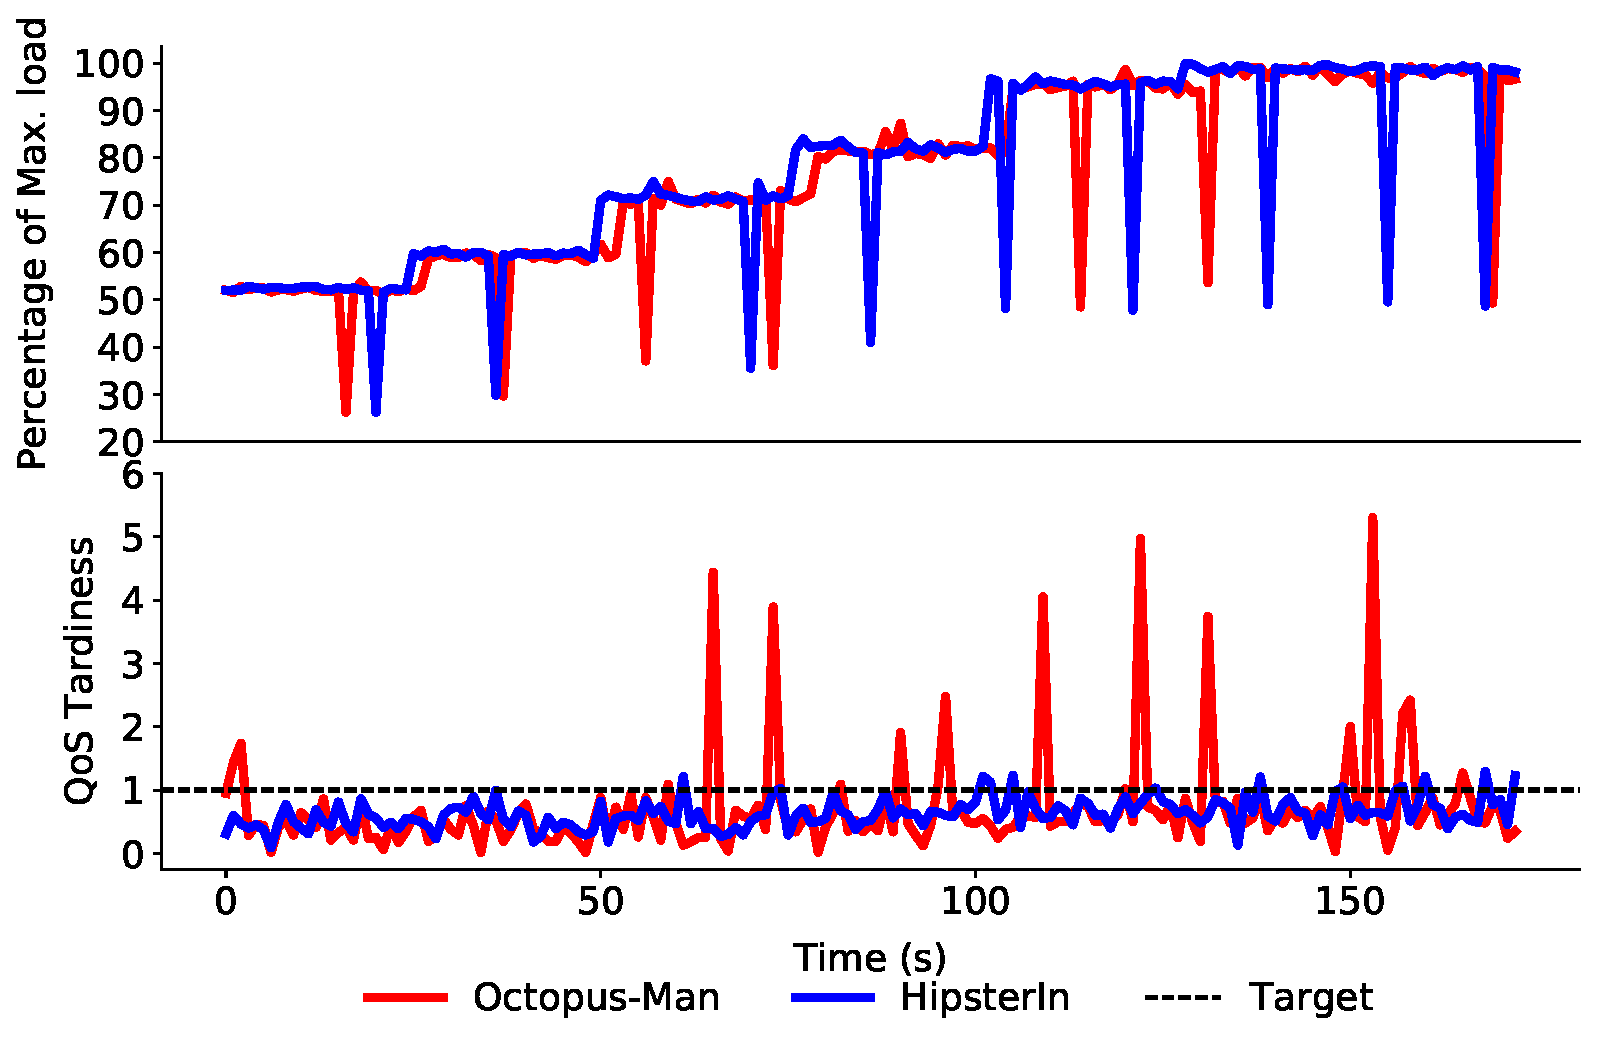
\includegraphics[width=0.7\linewidth]{Chapter4/Figs/detail_responsiveness.eps}
    \caption[Responsiveness to load change of HipsterIn and Octopus-Man]{\captitle{Responsiveness to load change of HipsterIn and Octopus-Man.} Percentage of Max. load, and Tail latency (QoS Tardiness) running Memcached with HipsterIn and Octopus-Man.}
	\label{fig: responsivenesstoloadchange}
\end{figure}



\paragraph*{Impact of learning time.} HipsterIn aims to deliver the best balance
between QoS guarantee and energy reduction compared to heuristic policies (Table~\ref{tab:
summarytable-hipster}). In practice, to best optimise for energy efficiency, and to improve QoS,
HipsterIn needs a short learning phase. Figure~\ref{fig: learningqos} shows the QoS
guarantee and energy distribution smoothed over \SI{100}{\second} intervals using the
Savitzky--Golay filter~\citep{Krishnan:2013:SOS:2710154.2710696} for Web-Search, for both
HipsterIn and Octopus-Man. Each data point in the graph refers to a 100-second interval.
The learning phase is set to \SI{200}{\second}. As can be seen, HipsterIn quickly learns
during the heuristic phase, which improves QoS guarantees. On the other hand, for
Octopus-Man, the QoS guarantees are consistently around the \SI{80}{\percent} mark, since
it does not use past decisions and their associated effects to improve the future
decisions. 

\begin{figure}[t]
    \centering
    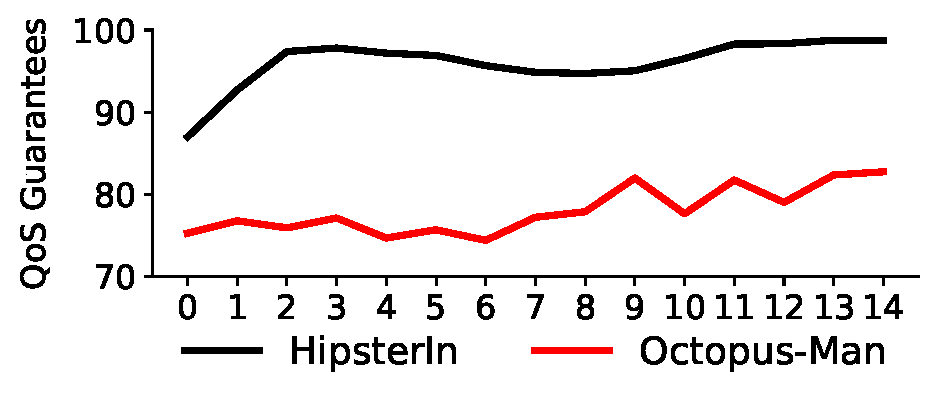
\includegraphics[width=0.8\linewidth]{Chapter4/Figs/learningqos.eps}
    \caption[QoS Guarantees of HipsterIn and Octopus-Man]{\captitle{QoS Guarantees of HipsterIn and Octopus-Man.} Each data point represents the QoS guarantees over \SI{100}{\second} intervals.}
    \label{fig: learningqos}
\end{figure}

\paragraph*{Impact of bucket sizes.} Figure~\ref{fig:loadbucket-qos-websearch} shows
the impact on QoS and energy savings when varying the load bucket sizes in Hipster. The
$x$-axis represents the bucket size, expressed as the percentage of maximum load. Each bar
in the figure ($y$-axis) represents the QoS violations and energy reductions normalised to
Static (all big cores). Using a large bucket size forces Hipster to use the same core
configuration across a wide range of loads, whereas using a small bucket size allows
fine-grained control. A small bucket size therefore improves the energy savings, but it
tends to cause rapid changes in core configuration for small changes in load, and doing so
incurs a larger number of QoS violations. On the other hand, larger bucket sizes provide
better QoS guarantee but lower energy savings, because they categorise large variations in
load into a single load bucket. Therefore, in tuning Hipster, we empirically determine the
bucket size to maximise energy savings subject to at least \SI{98}{\percent} QoS guarantee.

\begin{figure}[t]
\centering
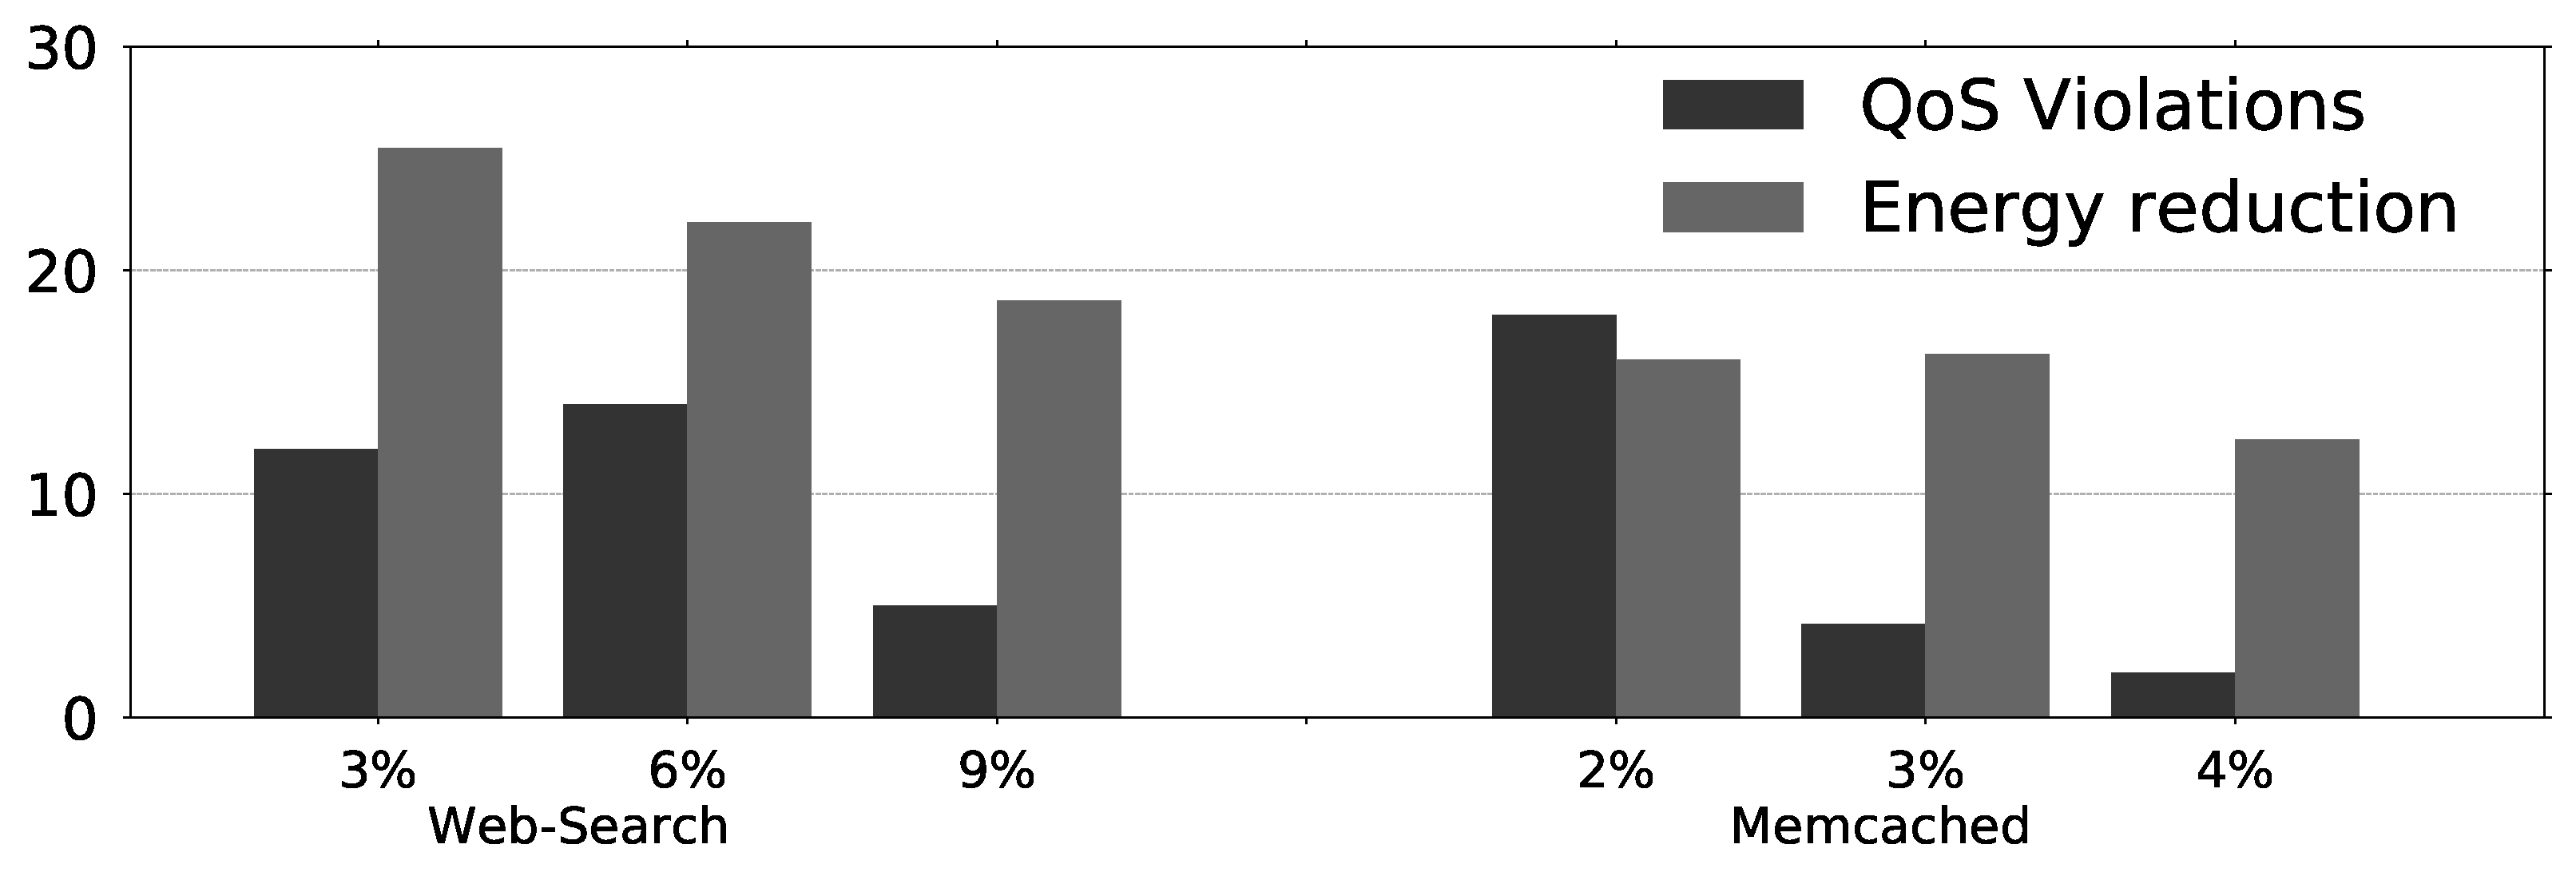
\includegraphics[width=0.95\linewidth]{Chapter4/Figs/bucketsize-qos-power.eps}
    \caption[Impact of bucket size on HipsterIn]{\captitle{Impact of bucket size.} QoS guarantees and energy savings normalised to static (all big cores) on Web-Search and Memcached.}
    %for HipsterIn QoS guarantees, and energy savings,normalised to static (all big cores) on Web-Search and Memcached.}
\label{fig:loadbucket-qos-websearch}
\end{figure}

\paragraph*{Optimising the lookup table size} Table~\ref{fig:sizehipster} summarises the
QoS guarantee, number of configurations per load bucket, and number of configurations for
Memcached and Web-Search with unoptimised and optimised lookup tables. We quantify the
reduction in lookup table size by assessing the number of configurations stored for each
load bucket at the end of the execution. As shown in Table~\ref{fig:sizehipster}, the
optimised lookup table saves \SI{90}{\percent} of the memory footprint while providing
similar QoS guarantee to unoptimised lookup table because, it only stores those
configurations that have been explored in the learning phase and in the exploitation
phase, the size of the table is further reduced by keeping only the top five
configurations with the highest reward. This is possible, as the configurations explored
at a given load level for a particular application are chosen from only a subset of the
configurations in the learning phase instead of random solutions as in Q-Learning.

\begin{table*}[t]
\centering
\ra{1.3}
\setlength{\tabcolsep}{5pt}
%{\def\arraystretch{2}\tabcolsep=10pt

    \caption{Results of the table size optimisation in Hipster} 
    \begin{tabular}{@{}llllr@{}}
        \toprule
                                                            &  Lookup Table           & Memcached	         & Web-Search  \\
        \midrule
        \multirow{2}{*}{QoS Guarantee (\%)}                 & Unoptimised    & 99.4                 & 96.5 \\
                                                            & Optimised      & 99.2                 & 96.0 \\
        \multirow{2}{*}{\# of config./load bucket}          & Unoptimised    & 13                   & 13  \\
                                                            & Optimised      & 5                    & 5 \\
        \multirow{2}{*}{Table size (elements)}              & Unoptimised    & 1344 (0\% savings)         & 392 (0\% savings) \\
                                                            & Optimised      & 120  (91.1\% savings)         & 35 (91.1\% savings)\\
                                                            
%        \multirow{2}{*}{Table Size in \SI{}{\kilo\byte}}    & Unoptimised    & 10.7                 & 10.7 \\
%                                                            & Optimised      & 0.9                  & 0.9 \\
        \bottomrule
    \end{tabular}    
    \label{fig:sizehipster} 
\end{table*}


\subsection{HipsterCo Results}
\label{subsec: coalloc}

\looseness -1 This section evaluates the effectiveness of HipsterCo, as a policy for
collocating a single latency-critical workload and a mix of batch workloads.  The
objective is to maximise the throughput of the batch workloads while satisfying QoS of the
interactive workloads.

Figure~\ref{fig:coallocaaaa} shows the QoS guarantee (top), throughput (middle) and energy
consumption (bottom) for Web-Search collocated with batch workloads, managed by
Octopus-Man and HipsterCo. All figures are normalised to a static mapping that allocates
the latency-critical workload to the two big cores and the batch workloads to the four
small cores. The number of running batch workloads is equal to the number of cores not
utilised by Web-Search. We report the system throughput by aggregating the IPS of all
batch programs. 

As shown in the top plot of Figure~\ref{fig:coallocaaaa}, HipsterCo consistently delivers
94\% QoS guarantees, whereas Octo\-pus-Man has much lower QoS guarantees of
\SI{76}{\percent}. This is because Hipster learns from the QoS behaviour and performance
history and is able to jump directly to a core mapping and DVFS state that satisfies QoS.
As a result, it incurs fewer core migrations compared with  Octopus-Man (see
Section~\ref{subsubsec: web-search results}), so it achieves superior QoS guarantees. 

\begin{figure}[ht]
    \centering
    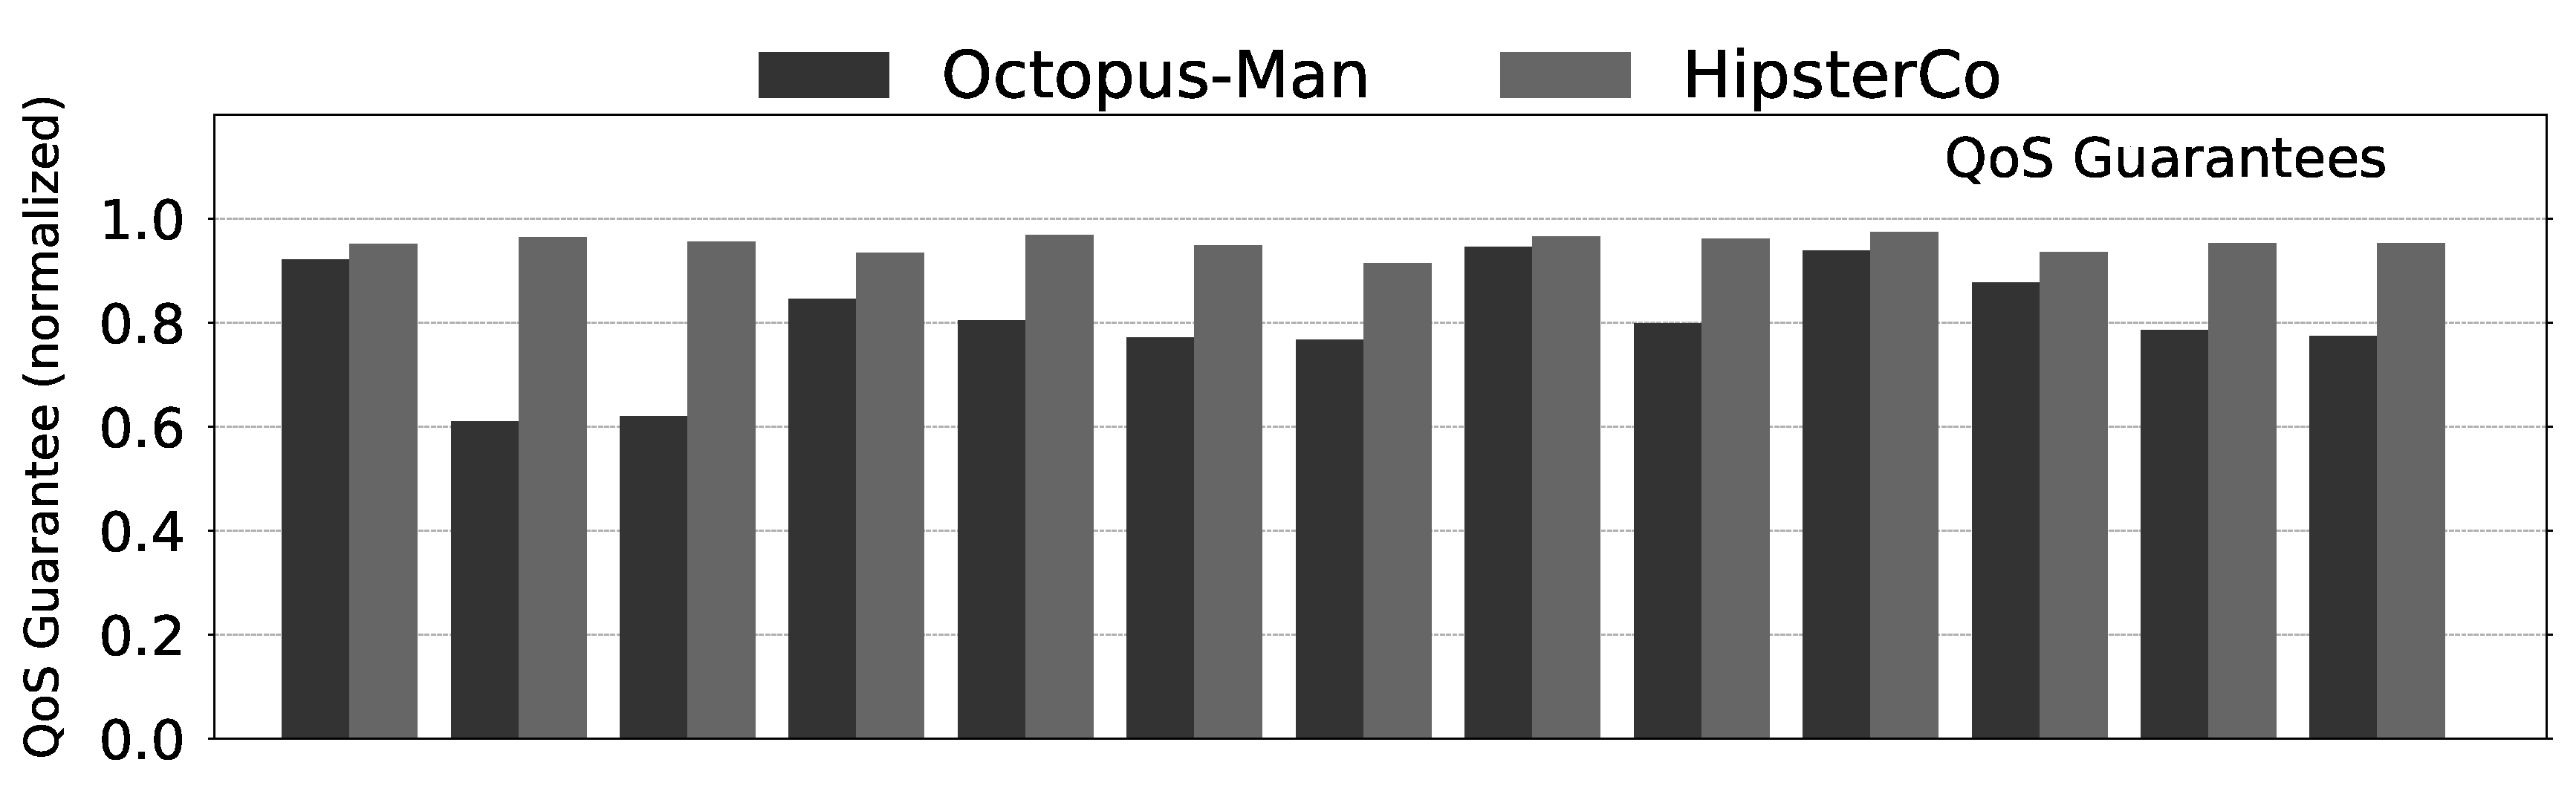
\includegraphics[width=0.9\linewidth]{Chapter4/Figs/guarantees_throughput_coalloc_without_yaxis.eps}
    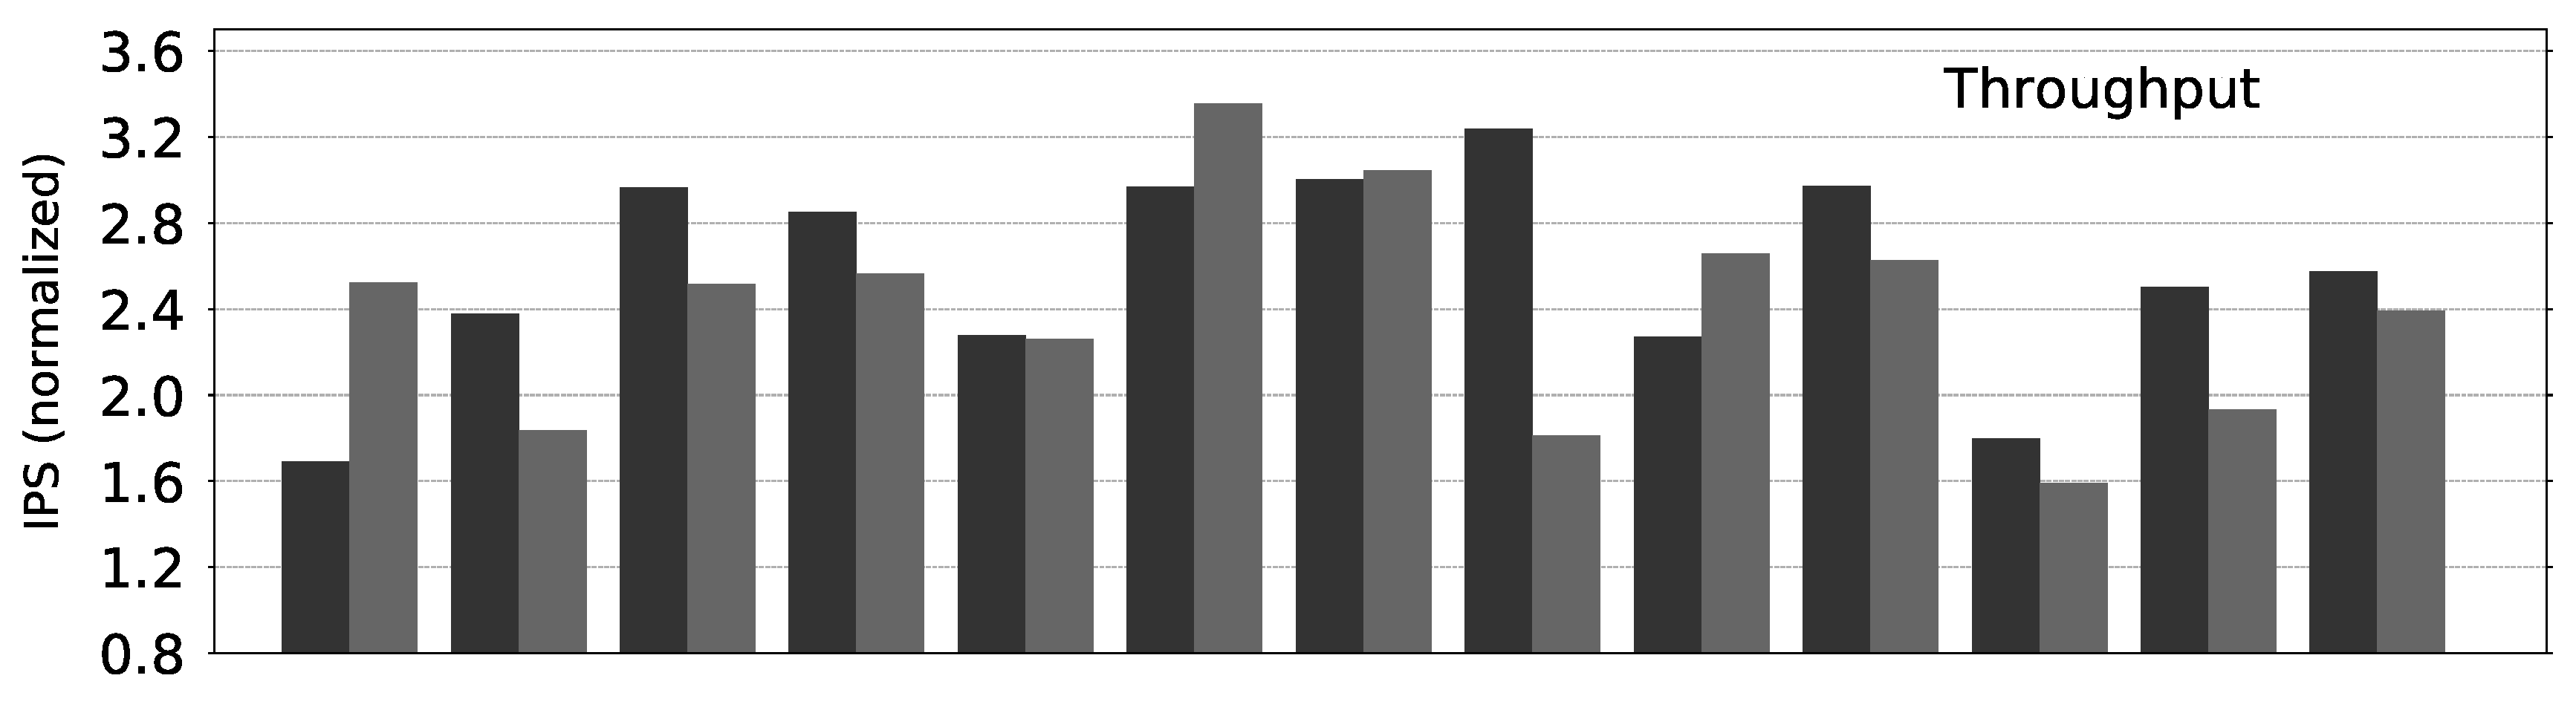
\includegraphics[width=0.9\linewidth]{Chapter4/Figs/throughput_coalloc_without_legend_axis.eps}
    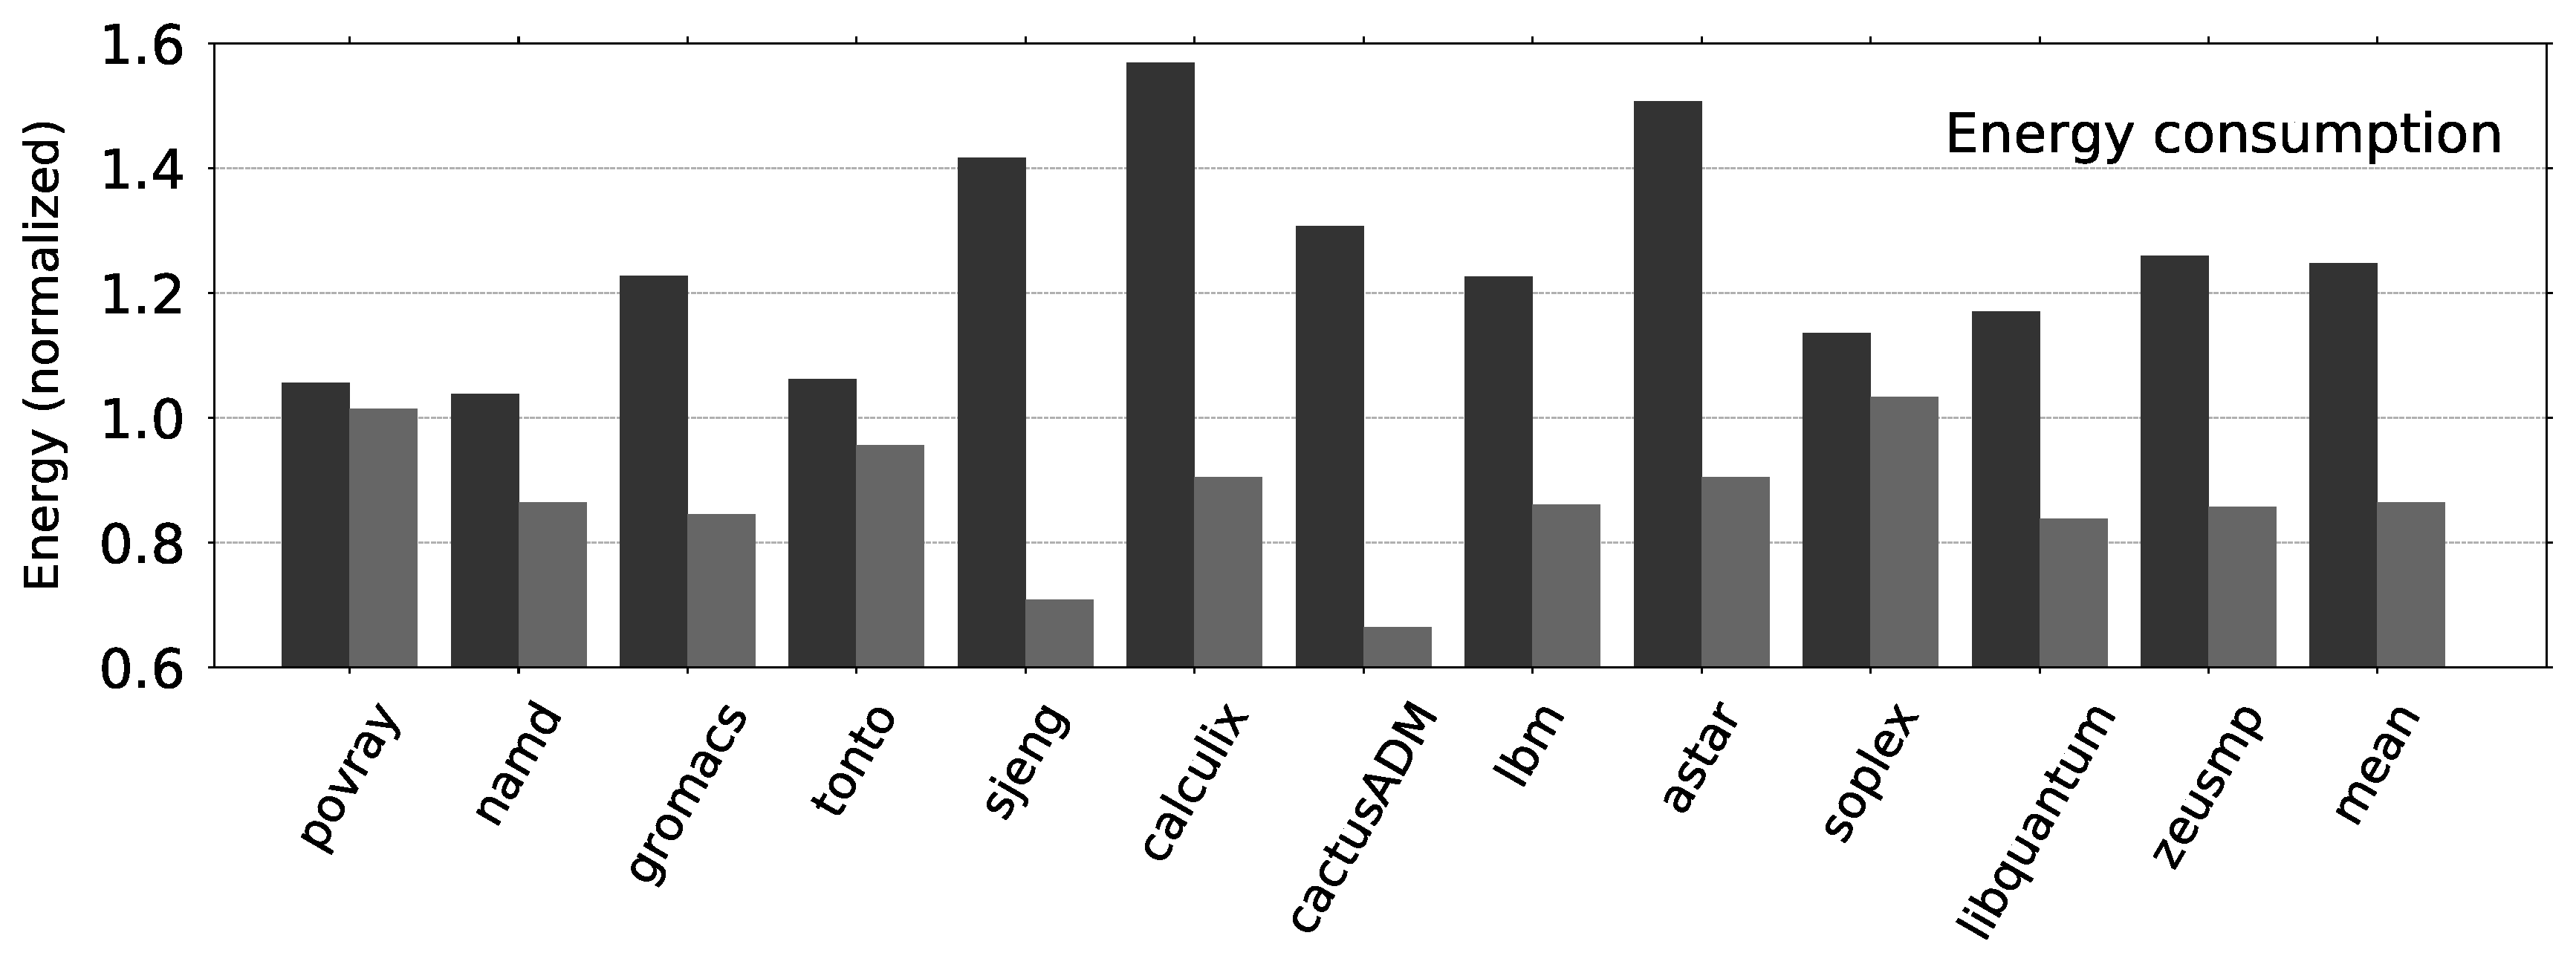
\includegraphics[width=0.9\linewidth]{Chapter4/Figs/energy_coalloc_withoutlegend.eps}

    \caption[Collocation of interactive and batch workloads with HipsterCo]{\captitle{Collocation of interactive and batch workloads with HipsterCo.} QoS guarantee (top), Throughput improvement (middle) and Energy consumption (bottom) when Web-Search is collocated with batch workloads. The results are normalised to static all big cores. }

\label{fig:coallocaaaa}
\end{figure} 

\looseness -1 As shown in the middle plot of Figure~\ref{fig:coallocaaaa}, for all
benchmarks, Hipster and Octopus-Man deliver much high\-er throughput compared to static
mapping, with an average of $2.3\times$ and $2.6\times$ improvement, respectively. Both
task managers improve performance compared with the static mapping because they migrate
the latency-critical workload to small cores during periods of low load, allowing the
batch workloads to run on big cores (which can be $2.6\times$ more powerful than small
cores).  For \emph{Calculix}, a compute-bound application, HipsterCo achieves the highest
throughput improvement over static of $3.35\times$, and for \emph{libquantum}, a
memory-bound program, the least improvement is still $1.6\times$.  

As shown in the bottom plot of Figure~\ref{fig:coallocaaaa}, HipsterCo reduces the energy
consumption to an average of \SI{80}{\percent} of static, whereas Octopus-Man increases
energy to an average of $1.2$ times that of static. This is because, as shown in
Figure~\ref{fig:octomancomp}, Hipster explores a wider range of core configurations,
including DVFS settings and mixing core types. In contrast, Octopus-Man only allows the
latency-critical workload to occupy a single cluster and each cluster is set to the
highest DVFS. 

HipsterCo sometimes chooses a different performance--energy trade-off than Octopus-Man.
An example is \emph{lbm}, a memory bound workload, for which HipsterCo delivers
\SI{40}{\percent} the throughput of Octopus-Man, but \SI{31}{\percent} lower energy.
There are two main reasons for this.  Firstly, when HipsterCo uses DVFS for the
latency-critical workloads, this DVFS setting also applies to batch workloads running in
the same cluster, reducing both batch throughput and system energy. Secondly, HipsterCo
sometimes uses a larger number of cores at lower DVFS, leaving fewer resources available
for the batch workloads. As a result, on average, HipsterCo marginally reduces performance
(by \SI{7}{\percent}) but it delivers energy savings of \SI{33}{\percent}, both compared
with Octopus-Man.
